\section{Description of proposed model}
The proposed model is a model for a simplistic library system. It represents a typical simple business application 
with some simple business processes supported by a database.

%--------------------------------------------------------------------------------------

\subsection{Rationale for choosing such a model}

\begin{itemize}
  \item in its default form it is very simple, without being overly academic, in nature, i.e.\ it is similar in nature to many
enterprise systems,
  \item people have generally a reasonable understanding of what would be required of a simple library system and the
domain concepts are generally accessible,
  \item it can be easily extended into a larger model which contains more elements of typical enterprise systems like 
    \begin{itemize}
		\item different presentation layers and access channels (web, mobile devices, web services, ...),
      \item it can be increased to include integration requirements (e.g. to book vendors, to other libraries, ...),
      \item it can be evolved to support electronic or paper based provision of electronically sourced and generated
material,
	 \end{itemize}
      \item common quality requirements like security, auditability, reliability and scalability may be applied to this model.
      \item it is suited to be implemented across different architectures and technologies (e.g., JavaEE, SOA, Clound 
				computing, ...)
\end{itemize}

%--------------------------------------------------------------------------------------

\subsection{Scope of model}
The scope of the initial model is purposefully kept very constrained. The system must support registration of library
members, uptake of items into the libraries inventory and loaning of library items. An overview of the scope of the system is
shown in Figure \ref{libraryScope_fig}

 \begin{figure}[htb]
  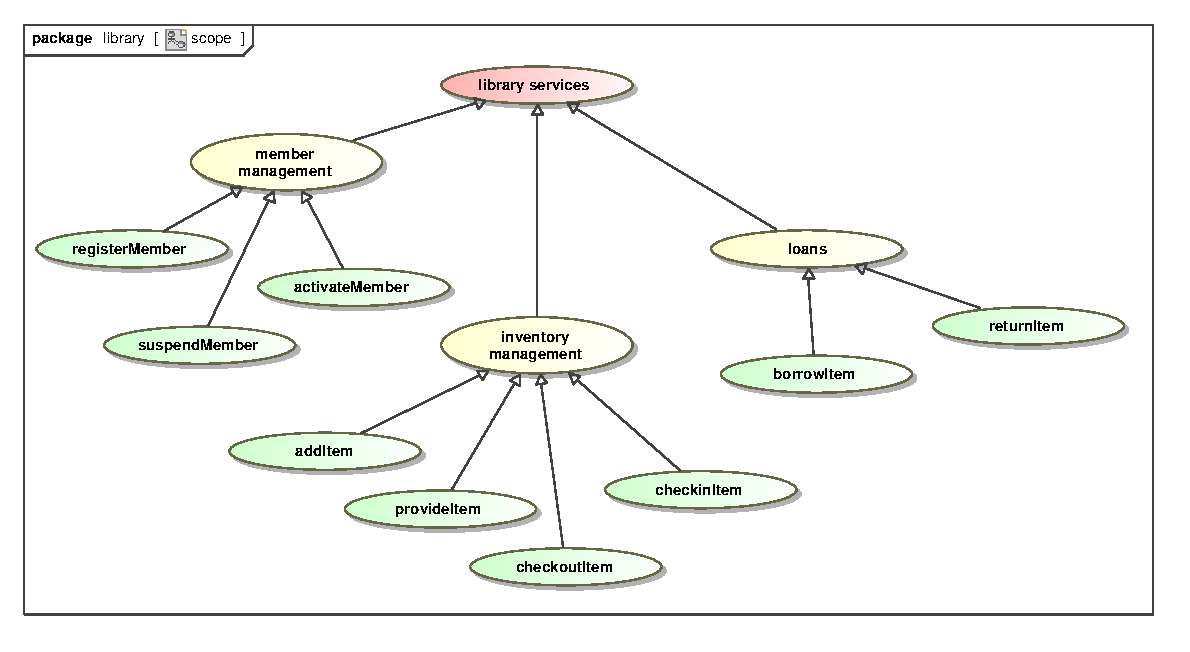
\includegraphics[width=1.0\textwidth]{scope}
 \caption{Scope of the library system.\label{libraryScope_fig}}
 \end{figure}
